Разработанная система является полностью статическим веб приложением, не имеющем необходимости в стороннем веб-сервере, обслуживающим пользовательские запросы, за исключением выдачи скомпонованных
статических ресурсов (файлов разметки, скриптов, каскадных таблиц стилей, файлов конфигурации). Данный подход одновременно и облегчает поддержку приложения (ввиду того, что существует возможность
распределенного хостинга ресурсов системы, нет нужды в хостинге всех ее частей на едином сервере, поскольку все взаимозависимости между ресурсами были ликвидированы на этапе компоновки), однако
уменьшает возможности по более гранулярному контролю за доступом пользователей к компонентам системы, не позволяя достичь точечной активации различного функционала для различных пользователей, что
потенциально может стать полезной функцией при монетизации подобного приложения.

Исходя из вышеуказанных соображений, целесообразно развитие серверного компонента системы, позволяющую выполнять ряд задач, связанных с высокопроизводительной обработкой графики, а именно:
\begin{itemize}
\item рендеринг сцен трехмерной графики на сервере по-требованию (On-demand) клиентского компонента приложения, что позволяет реализовать быстрый децентрализованный рендеринг на базе облачных
сервисов (MS Azure, AWS), позволяя пользователям относительно слабых компьютеров или переносных у-стройств рендерить детализированную трехмерную сцену в высоком разрешении за малый промежуток
времени.
\item удаленное хранение пользовательской конфигурации, что позволяет по-льзователям работать на разных устройствах без потери сессии работы с трехмерной моделью;
\item доступ к централизованному хранилищу трехмерных моделей, шейдеров, ресурсов и плагинов для приложения.
\end{itemize}

Поскольку само приложение-редактор выполнено в виде целиком самостоятельного веб приложения, у него нет строгих требований к использованному стеку серверных технологий. В случае реализации
серверного приложения, приложение станет гибридным и более недопустим его хостинг на статической платформе веб страниц, например GitHub Pages. Также один из потенциальных подходов к разработке
удаленной части приложения - использование микросервисной (рисунок \ref{figure:outro:microservices}) (без серверной -- serverless) архитектуры на хостинге Microsoft Azure Functions, Amazon Lambdas либо на легковесном фреймворке 
serverless stack StdLib. Последний подход позволяет более тесно интегрировать приложение в облачные сервисы и позволяет легче расширять возможности вычислительной сети по мере необходимости и
роста количества пользователей, а также использовать близкие к веб-среде технологии и языки программирования и в среде серверов (потому как Azure Functions\cite{azure} и StdLib\cite{stdlib} осуществляют поддержку node.js
совместимых модулей обработки серверного поведения).

\begin{figure}[ht]
\centering
  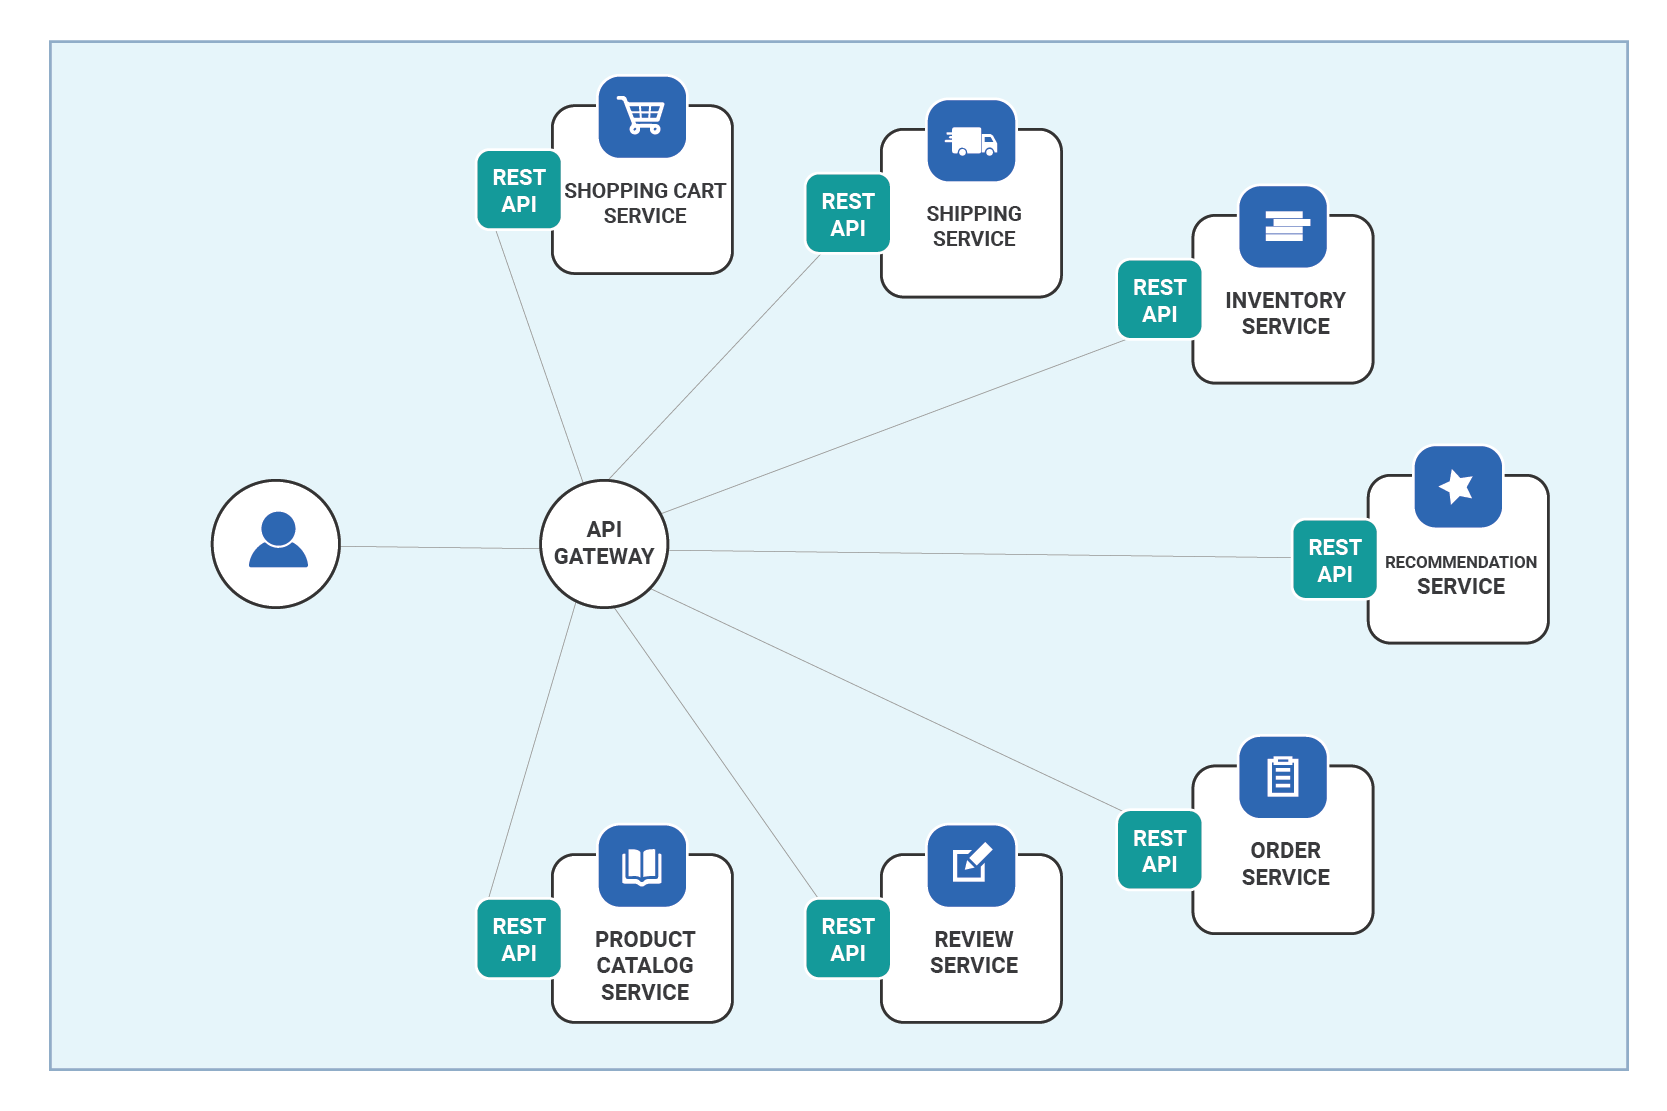
\includegraphics[scale=0.8]{microservices.png}
  \caption{Пример структуры приложения на базе микросервисной архитектуры}
  \label{figure:outro:microservices}
\end{figure}

К плюсам децентрализованного микросервесного подхода можно отнести:
\begin{itemize}
\item относительную переносимость решения;
\item усложнение несанкционированного доступа к приложению
\item потенциальную прогрессивную модель монетизации
\item возможность постепенной разработки и централизованной доставки обновлений
\item облачное резервное копирование работы пользователя в автоматическом режиме
\end{itemize}

Тем не менее, микросервисный подход имеет и ряд недостатков:

\begin{itemize}
\item приложение доступно лишь через веб, то есть требует постоянный доступ к интернету;
\item затраты на поддержку серверов приложения;
\item несколько более низкая производительность по сравнению с классическим подходом.
\end{itemize}

Также в самом клиентском приложении отсутствует некоторые из распространенных возможностей большей части редакторов трехмерных моделей, а именно, возможности цифровой скульптуры.
Поскольку разработанное приложение большей частью ориентировано на создание моделей, построенных на основе примитивов, оно малопригодно для создания органично-выглядящих моделей,
таких как изображения животных или людей. Реализация набора инструментов для цифровой скульптуры позволит восполнить этот недостаток приложения и дать пользователям возможность
использовать его для создания более полного набора объектов геометрии.

Основные инструменты для цифровой скульптуры, разработка которых требуется для эффективного использования данного функционала:
\begin{itemize}
\item инструмент создания совместимых со скульптором примитивов;
\item набор меню пользовательского интерфейса для работы с системой цифровой скульптуры;
\item набор сервисов манипуляции геометрией объектов, позволяющих динамическое увеличение детализации трехмерных моделей в процессе работы, поддерживающий работу со всеми
существующими примитивами.
\item набор правил, обрабатывающих поведение выталкивания вершин из трехмерной модели (отличный от стандартного менаханизма, описанного в модуле ModelLoopExtruder (описанный,
в разделе \ref{sub:theory:components:geometry}))
\end{itemize}

Проблема реализации механизмов цифровой скульптуры заключается в том, что при работе со стандартными средствами работы с примитивами, производимая трехмерная модель может быть
легко редактирована с помощью средств манипуляции замкнутыми граничными циклами (Edge Loops), который становится недоступен в случае произвольной манипуляции моделью, как например в случае
редактирования средствами цифровой скульптуры.

Также средства цифровой скульптуры в большинстве случаев порождают модели с большим количеством треугольников, которые можно оптимизировать средствами бамп-маппинга, однако этот
механизм сложно реализуем в реальном времени и на устройствах с потенциально слабой производительностью, что может потенциально ограничивать часть пользователей (например, пользователей
мобильных устройств или очень слабых компьютеров). Проблема указанной выше реализации состоит в том, что при переходе к использованию механизмов цифровой скульптуры, изменения, вносимые
в трехмерную модель, становятся необратимы, что значительно уменьшает производительность системы в случае работы с такими моделями. Данная проблема может быть решена путем введения двух
различных форматов работы со скульптурами, то есть разделения механизмов цифровой скульптуры и классического трехмерного моделирования, основанного на подразделении вершин и линейных
преобразованиях над граничными циклами.